\documentclass[a4paper,12pt]{article}
\usepackage{template}

\usepackage{algpseudocode}
\usepackage{algorithmicx}
\usepackage{longtable}

\begin{document}

\section{Lecture 1}
\subsection{Neural cell (Neuron)}
\begin{tabular}{p{4cm}p{9cm}p{5cm}}
Main components	& A typical neural cell consists of dendrites, the soma (aka pericaryon) and one axon. The axon can have many branches however.	& There are about 10'000 neurons per mm$^3$\\
Soma		& The soma contains various organelles, such as endoplasmatic reticula or mitchondria. Among other substances, it produces Neurotransmitters.	& The soma is about 5 to 100 $\mu$m in diameter.\\
Dendrites	& Dendrites collect the information from other neurons. The dendritic tree of a single neuron can be connected with up to 200'000 other neurons.	& In one mm$^3$, there are about 5m dendrites.\\
Axon		& The axon is more or less branched and each branch ends in presynaptic terminals. 	& Length: 1 $\mu$m - 1 m. Diameter: 0.5 - 10 $\mu$m. In one mm$^3$, there are about 5km axons.\\
Synapses	& The synapse is an interface, through which chemical information can be transmitted from one cell (axon) to the other (dendrite). 	& A neuron has about 10'000 synapses with other neurons. The human brain has about $10^{15}$ synapses.
\end{tabular}
\subsection{Nervous system}
\begin{tabular}{p{4cm}p{15cm}}
Definition	& The nervous system coordinates the activity of all body parts and transmits information from and to them. In most animals, the nervous system consists of the central nervous system (CNS) and the peripheral nervous system (PNS). The presence of \textbf{neurons and glial cells} is characteristic for the nervous system. The brain consists of about $10^{11} - 10^{12}$ neurons.\\
CNS		& The CNS is the part of the nervous system that receives information and coordinates activity of all parts of the body. It consists of the \textbf{brain and spinal cord (R�ckenmark)}. Sometimes, the retina and the cranial nerves (Hirnnerven) are added to the CNS. Brain and spinal cord are protected by the skull and the backbone respectively.\\
PNS		& The PNS consists of the nerves outside the CNS. Its main function is to connect the CNS to the limbs and organs. The PNS is not protected by bones. As an example, the PNS includes motor nerves.
\end{tabular}


\section{Lecture 2}

\subsection{Transport through membranes}
\begin{longtable}{p{4cm}p{15cm}}
Cellular membrane	& 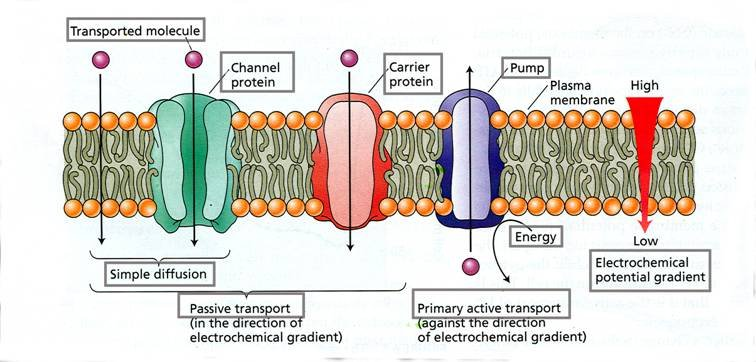
\includegraphics[width = 14cm]{neuroinf_membrane.jpg}\\
Phospholipids		& The membrane consists of a bilayer of phospholipids. The heads are charged and hydrophil. The tails are oily and hydrophob.\\
Passive transport	&\\
- Simple diffusion	& Small, lipophile and non-polar molecules can diffuse through the membrane. They are governed by differnces in concentration and / or charge.\\
- Channel protein	& Within the membrane, there are channels (channel proteins) which have aminoacids at their interior. Therefore, small polar or charged particles like ions can get transported through these channels. Typically, the channels need to be opened chemically, electrically or mechanically.\\
- Carrier protein	& A special carrier protein binds with a certain molecule. The carrier protein changes its conformation at binding. That way, the molecule gets carried through the membrane. There are carrier proteins which can only one or two molecules at once.\\
Active transport	&\\
- Sodium-Potassium Pump	& \begin{itemize}
                       	  	\item The Sodium-Potassium-ATPase (3 Na$^+$ / 2 K$^+$ - ATPase) aka Sodium-Potassium pump is transport protein in the membrane.
				\item The pump is opened at the inside. Three Na$^+$ are taken into the pump.
				\item The pump changes its conformation which leads to the release of Na$^+$ ions to the extracellular fluid. The processes which lead to the conformation need energy, which is yielded by the ATP.
				\item From the ECF, two K$^+$ kations are taken into the pump. Again, a conformational change is invoked and the two K$^+$ are expelled into the ICF.
				\item Per cycle, the pump removes one charge unit from the ICF. Thereby it helps maintaining a resting potential.
                       	  \end{itemize}\\
Typical ion concentrations in body		& \begin{tabular}{lll}
			    Ion		& Interior (mM)	& Exterior(mM)\\\hline
			    Na$^+$	& 15		& 150\\
			    K$^+$	& 150		& 5\\
			    Ca$^{2+}$	& 0		& 2.5\\
			    Cl$^-$	& 110		& 10\\
		\textbf{large Anions}	& \textbf{65}	& \textbf{2}
			  \end{tabular}\\
Gibbs-Donnan-Equilibrium	& Large Anions cannot be transported through the membrane by any means. Also, some ions (potassium) might have a bigger permability. This influences the diffusion of the other ions. Both ICF and ECF must be electrically neutral. At equilibrium, the concentrations of the inner and outer ions are therefore not equal. As a consequence, a persistent potential difference arises.\\
Cellular membrane	& 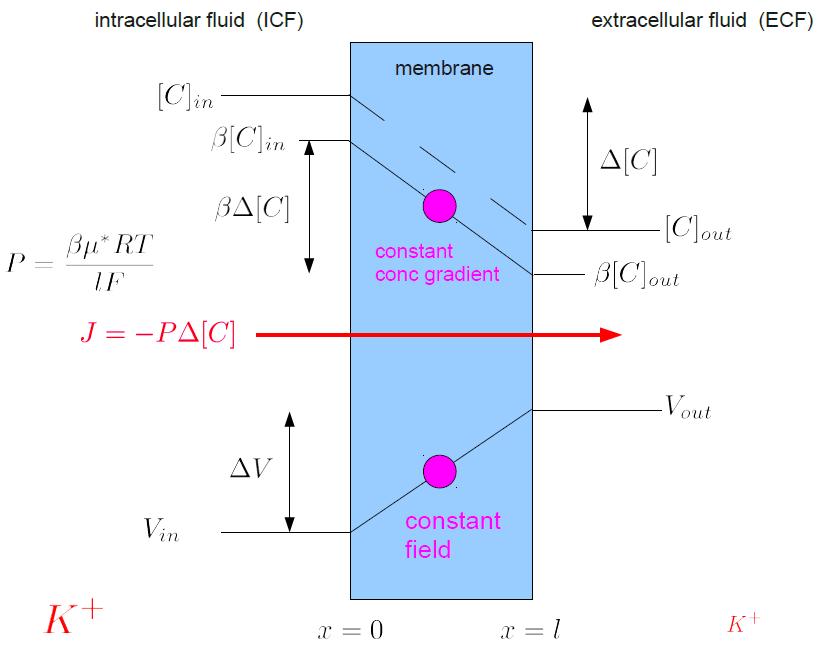
\includegraphics[width = 14cm]{neuroinf_cell_membrane_transport.png}\\
\end{longtable}
\subsection{Maths}
\begin{tabular}{p{4cm}p{15cm}}
Fick's law of diffusion		& \begin{tabular}[t]{l}
				    $\boxed{J_{diff} = -D \frac{ \partial [C]}{\partial x}}$\\
				    $J_{diff}:$ diffusion flux $[$molecules$ / (s \cdot cm^2)]$\\
				    $D:$ diffusion coefficient $[cm^2/s]$\\
				    $[C]:$ concentration of species $[molecules/cm^3]$
				  \end{tabular}\\
Ohm's law of drift		& \begin{tabular}[t]{l}
				    $\boxed{J_{drift} = \partial_{el} E = -\mu z [C] \frac{\partial V}{\partial x}}$\\
				    $J_{drift}:$ drift flux $[$molecules$ / (s \cdot cm^2)]$\\
				    $\partial_{el}$: electrical conductivity $[$molecules$ / (V \cdot s \cdot cm)]$\\
				    $E = -\partial V / \partial x$: electric field $[V/cm]$\\
				    $V:$ electric potential\\
				    $\mu:$ mobility $[cm^2 / (V \cdot s)]$\\
				    $z:$ valence of ion
				  \end{tabular}\\
Einstein Relation		& \begin{tabular}[t]{l}
				    $\boxed{D = \frac{k_B T}{q} \mu = \frac{RT}{F} \mu}$\\
				    $q: $ charge of the molecule [Coulombs]
				  \end{tabular}\\
Nernst-Planck-Equation		& $\boxed{I = J_{tot} \cdot zF = -\left(\mu z^2 F[C] \frac{\partial V}{\partial x} + \mu z RT \frac{\partial [C]}{\partial x}\right)}$\\
Nernst-Equation			& \begin{tabular}[t]{l}
				    Resting potential: Use NPE with no net flux $\Rightarrow I = 0$\\
				    $V_2 - V_1 = -\frac{RT}{zF} \ln \frac{[C]_2}{[C]_1}$\\
				    $\boxed{V_2-V_1 = -\frac{RT}{F} \ln \frac{[C]_{in}}{[C]_{out}}}\quad$ for $ z=1$
				  \end{tabular}\\
				& With the Nernst-equation, we can calculate the voltage difference arising by the Donnan-Equilibrium (aka the resting potential).\\
Prefactor			& $\boxed{\frac{RT}{F} = 26.7 $mV at T $= 37^{\circ}$C$}$ To be used with the natural logarithm (Nernst-equation)\\
				& $\boxed{\frac{RT}{F} \ln(10) = 61.5 $mV at T $= 37^{\circ}$C$}$ To be used with the base 10 logarithm (GHK equation)\\
Permeability			& \begin{tabular}[t]{l}
            			  	$P = \frac{\beta D}{l}$\\
					$\beta$: Water-membrane partition coefficient for ion $i$\\
					$l$: Thickness of membrane.\\
					$J = -P \Delta[C]$
            			  \end{tabular}\\
Goldman-Hodgkin-Katz Equation	& \begin{tabular}[t]{l}
				    $\boxed{\Delta V  = \frac{RT}{F}\cdot\log_{10}\frac{P_{\text{Na}}\cdot[\text{Na}^+]_a+P_\text{K}\cdot[\text{K}^+]_a+P_\text{Cl}\cdot[\text{Cl}^-]_i}
{P_\text{Na}\cdot[\text{Na}^+]_i+P_\text{K}\cdot[\text{K}^+]_i+P_{\text{Cl}}\cdot[\text{Cl}^-]_a}}$\\
				    P = Permeability, $\sum P_i = 1$\\
				    $\Delta V$ is the voltage difference between the interior and the exterior of a cell.
				  \end{tabular}\\
				& The GHK voltage equation is a generalization of the Nernst-equation.
\end{tabular}

\section{Lecture 3}
\subsection{Electrical properties of a cell}
\subsubsection{General ohmic model}
\begin{tabular}{p{4cm}p{15cm}}
Circuit representation of biological membrane	& 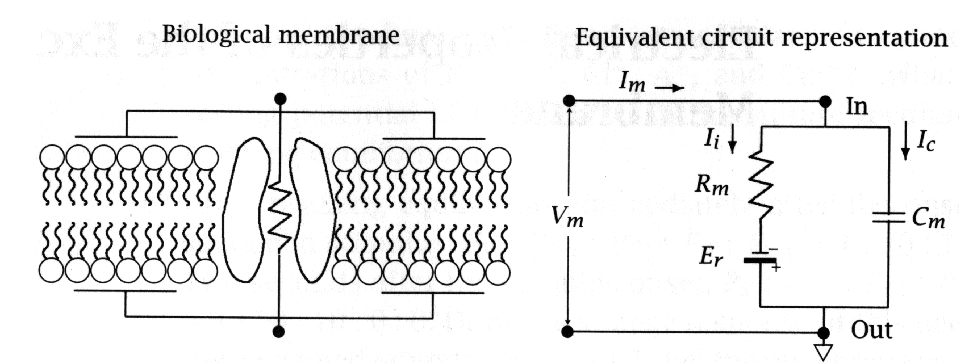
\includegraphics[width = 14cm]{neuroinf_biomembrane_as_circuit.png}\\
Capacitance $(C_m, V_m)$	& The capacitance is determined by the properties of the lipid bilayer (polar heads are conducting, apolar tails are isolating (dielectricum)) and is \textbf{fixed}.\\
Conductance $(g_m)$	& The conductance represents the various channels (carrier protein, channel protein, sodium-potassium pump), whose permabilities are \textbf{variable}. The conductance is of course inverse to the resistance $R_m$\\
Battery $(E_r)$		& The battery represents the resting potential arising by persistent concentration gradients. The resting potential is \textbf{fixed}.\\
Current $(I_m)$		& $I_m = C_m \frac{dV_m}{dt} + \frac{V_m-E_r}{R_m}$. Unless there is a arbitrary current from outside (for experiments), $I_m = 0$
\end{tabular}
\subsubsection{Ohmic model applied on neuron}
\begin{longtable}{p{4cm}p{15cm}}
Total current	& \begin{tabular}[t]{ll}
             	  $I_m$ 	& $= I_C + I_K + I_{Na} + I_{Cl}\quad I_m = $external current source\\
				& $= C_m \frac{dV}{dt} + g_k(V-E_k) + g_{Na}(V-E_{Na}) + g_{Cl}(V-E_{Cl})$
             	  \end{tabular}\\
Resting potential ($I_m = 0, \frac{dV}{dt} = 0$)	& $\boxed{V_{rest} = V = \frac{g_kE_k + g_{Na}E_{Na} + g_{Cl}E_{Cl}}{g_k + g_{Na} + g_{Cl}}}$\\
				& This is the GHK voltage equation in electrical terms.\\
Typical membrane parameters	& \begin{tabular}[t]{l|ll}
								& Independent of geometry	& for cylinder\\\hline
					    Diameter		& -				& $a = 20 \mu m$\\
					    Capacitance		& 1 $\mu F / cm^2$		& $c_m = C_m 2\pi a L \approx 10$ pF\\
					    Membrane Resistance	& $R_m = 10 k\Omega cm^2$	& $r_m = \frac{R_m}{2\pi a L} \approx 1 $G $\Omega$\\
					    Axial resistance	& $R_a = 100 \Omega cm$		& $r_a = \frac{R_a}{a^2 \pi}$\\
					    Time constant	& -				& $\tau = c_m r_m \approx 10$ ms
					  \end{tabular}\\
Current loss in axon	& \begin{tabular}[t]{p{14cm}}
			  There is an exponential decay of voltage due to leakages to the extracellular area. This decay can be modeled with the cable equation.\\
			  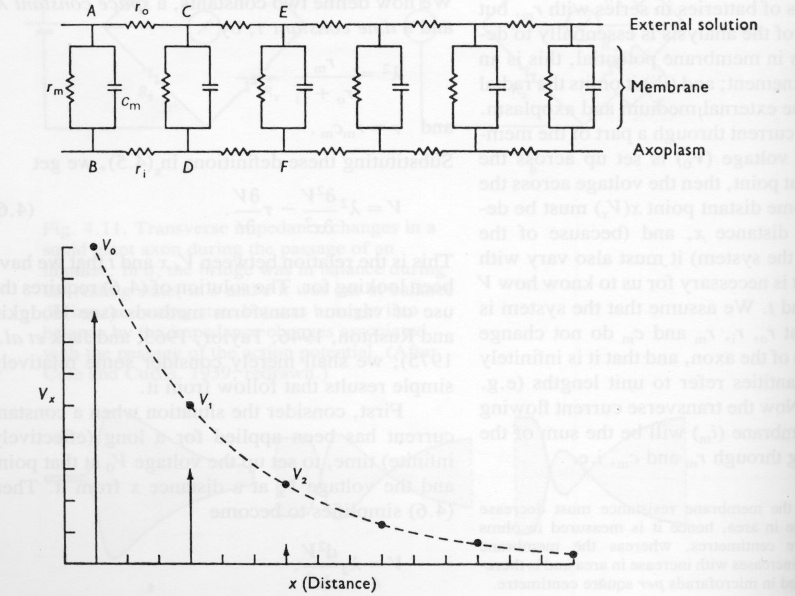
\includegraphics[width = 10cm]{neuroinf_voltagelossaxon.png}
			  \end{tabular}\\
Cable equation		& \begin{tabular}[t]{l}
			   $\boxed{\tau \left(\frac{\partial v}{\partial t} \right) = \lambda^2 \left( \frac{\partial^2v}{\partial x^2} \right) - v + r_m i_e}$\\
			   $\lambda = \sqrt{\frac{r_m}{r_a}} = \sqrt{\frac{a R_m}{2 R_a}}\qquad v = V-V_{rest}$\\
			   $i_e$: injected current\\
			   $r_m$: membrane resistance (geometry dependent)\\
			   $r_a$: axial resistance (geometry dependent)\\
			   $\lambda$: space constant. For $x=\lambda$, the voltage has decayed about an $e$-fold.
			  \end{tabular}\\
Stationary solution	& $\boxed{v(x) = \left( \frac{i_e R_{\lambda}}{2} \right) e^{-|x| / \lambda}}$\\
Remarks on $\lambda$& \begin{itemize}
				\item The bigger $\lambda$, the better (in terms of voltage transfer)
				\item The bigger the diameter, the bigger $\lambda$
				\item The bigger the membrane resistance, the bigger $\lambda$
				\item For a human membrane, $\lambda \approx 0.6$ mm
                           \end{itemize}
\end{longtable}
\subsection{Basic formulae}
\begin{tabular}{p{4cm}p{15cm}}
Ohm's Law	& $U = R \cdot I$\\
Capacitance	& $C = \frac{q}{U}$\\
Current and Capacitance	& $I = C \frac{dV}{dt}$\\
Conductivity	& $g = \frac{1}{R}$\\
Charging of a capacitor	& $\frac{I_{inj}}{g}(1-e^{-t/\tau}) + E$\\
Kirchhoff Current Law	& Inflow = Outflow at a node\\
Kirchhoff Voltage Law	& In every circuit, the sum of the voltages must be zero
\end{tabular}

\section{Lecture 4}
\begin{tabular}{p{4cm}p{15cm}}
Resting potential	& Due to concentration differences, caused by a selectively permeable membrane, there is a permanent voltage difference between the interior and the exterior of a neuron. The resting potential can be computed by the GHK equation, which depends on the conductances (permeability in the biological context) of the membrane w.r.t. each ion.\\
Conductance		& The conductance of a membrane is determined by the ion channels of the membrane. The permeability of the ion channel is not constant. Instead, there are ligand-gated, strech-activated, light-gated (mostly synthesized) and voltage-gated ion channels. Therefore, the conductance of a membrane w.r.t. an ion $X$ is not constant. Voltage-gated ion channels depend on the membrane potential. They give rise to positive feedback loops (see below) and are capable to trigger action potentials. That's why we want to look at voltage-gated ion channels. So, the conductance depends on the voltage and a certain time constant, i.e. $g_X = g_X(V,\tau_X)$\\
Action potential	& Since the conductances for different ions change not equally fast, the potential difference can vary from the resting potential. Typically, the potential rises sharply, then falls again, undershoots and levels out again at the resting potential. This process is called an action potential.\\
Threshold potential	& The threshold potential is the level which must be reached for an action potential to be triggered.\\
			& 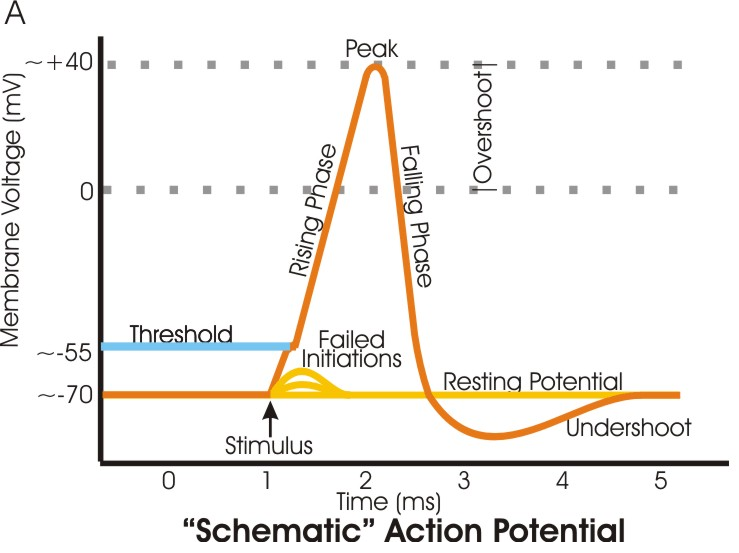
\includegraphics[width=12cm]{neuroinf_actionpotential.png}\\
\end{tabular}
\begin{longtable}{p{4cm}p{15cm}}
Membrane model	& 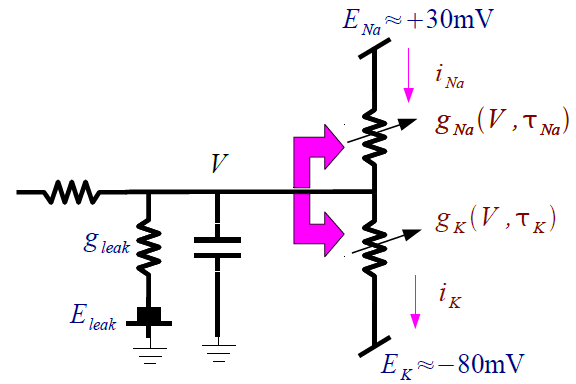
\includegraphics[width = 10cm]{neuroinf_membrane_as_circuit2.png}\\
		& The arrows indicate that the conductances depend on the voltage $V$. The capacitance is well-known, the subscript leak refers to the axon leakage and the resistance at the left refers to some dendrites or whatever.\\
Conductances w.r.t. Na$^+$ and K$^+$	& 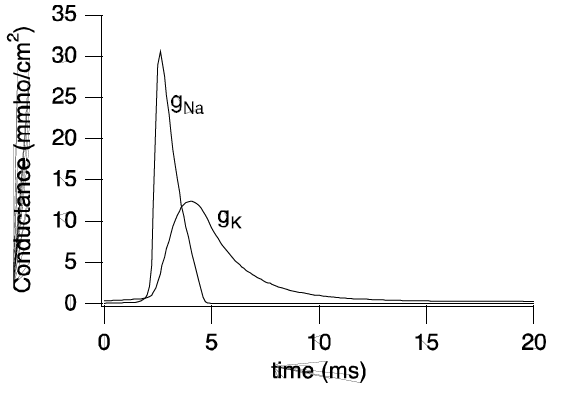
\includegraphics[width=8cm]{neuroinf_conductances.png}\\
Feedback loops	& If, for some reason (e.g. spike from other neuron), the membrane voltage increases (or decreases), the conductance for ion X rises (or falls) as well. This causes the X current to rise, which causes the membrane voltage to rise aka \textit{depolarization} (or fall aka \textit{hyperpolarization}) further and this causes the conductance to rise (or fall) further, resulting in a positive (or negative) feedback loop.\\
Action potential mechanism	& $\tau_{Na} < \tau_{K}$, that is, Sodium ions reacts faster on a voltage change than Potassium ions.\newline
		  If the membrane voltage change exceeds the threshold voltage, a \textit{positive feedback loop} w.r.t. Na$^+$ starts and Sodium ions enter.\newline
		  When Potassium reacts to the initial voltage change, the positive feedback loop ends and a \textit{negative feedback loop} w.r.t. K$^+$ starts and Potassium ions begin to leave the membrane. At this moment the maximal membrane potential is achieved.\\
Threshold potential value	& In this model, the threshold potential value is at the voltage where the Na$^+$ and the K$^+$ \textit{current} are equal, i.e. $V(I_{Na^+} = I_{K^+})$, because $\frac{dV}{dt}~ \propto ~ I$ and the feedback loop is about the increase or decrease, i.e. the \textit{change} in voltage.\\
Charge carriers	      & During the action potential, Sodium ions enter and Potassium ions leave the membrane. Hence, at the end of an action potential, the Na$^+$ and K$^+$ concentratios have changed. To restore the original ratio of ion concentrations, the ions are pumped back by the sodium potassium pump. This is a feasible task, since relatively few ions need to cross the membrane for the membrane voltage to change drastically.\\
Myelin	& Some axons are encapsulated by myelin, which is essentially a insulator $\Rightarrow \lambda$ becomes bigger! On the downside, it requires more space and myelinated regions cannot produce action potentials.\\
Ranvier-nodes	& Axons are not myelinated along their full length. Instead, regularly spaced unmyelinated patches, called the nodes of Ranvier, generate action potentials to reinforce the signal.\\
Termination	& Generally, the action potential ends in an axon terminal, where it leads to the release of neurotransmitters into the synaptic cleft. In addition, action potentials can also backpropagate into the dendrites.
\end{longtable}
\subsection{Hodgkin-Huxley equation}
In general, the Hodgkin-Huxley equation is again an equation which describes the membrane potential. Precisely, it describes the membrane voltage during the action potential by imposing time-dependent expressions for the conductances by a fit to experimental data.\\
\begin{tabular}{p{4cm}p{15cm}}
General form		& $C \frac{dV}{dt} + \bar{g}_K(V-E_K) + \bar{g}_{Na}(V-E_{Na} + \underbrace{\bar{g}_L (V-V_L)}_{generic leak} + I_{inj} = 0$\\
			& $\bar{g}_K = g_K n^4(t)\quad n(t) \in [0,1]$\\
			& $\bar{g}_{Na} = g_{Na} m^3(t)h(t)\quad m(t),h(t) \in [0,1]$\\
Fitting to experimental data	\\
- Potassium	& 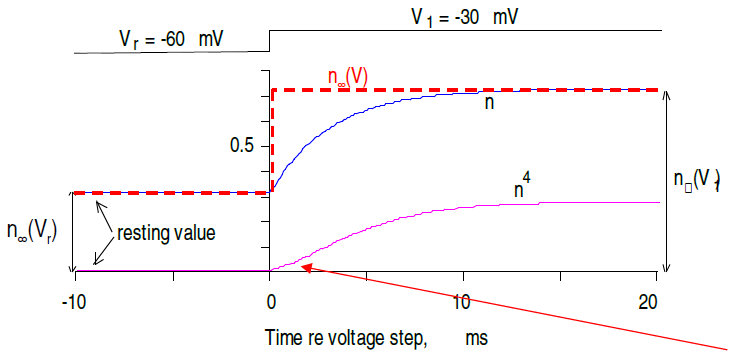
\includegraphics[width = 10cm]{neuroinf_hhm_n.png}\\
		& $g_K = \bar{g}_Kn^4$\\
- Sodium	& 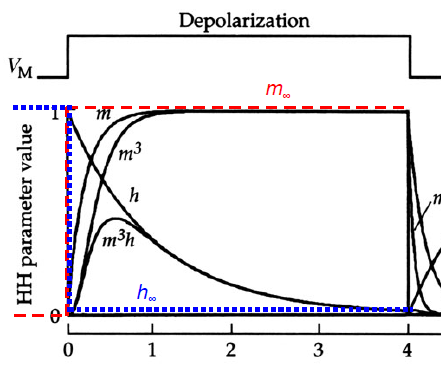
\includegraphics[width = 10cm]{neuroinf_hhm_mh.png}\\
		& $g_{Na} = \bar{g}_{Na} m^3h$
\end{tabular}



\section{Lecture 5}
\begin{longtable}{p{4cm}p{15cm}}
Synapse		& 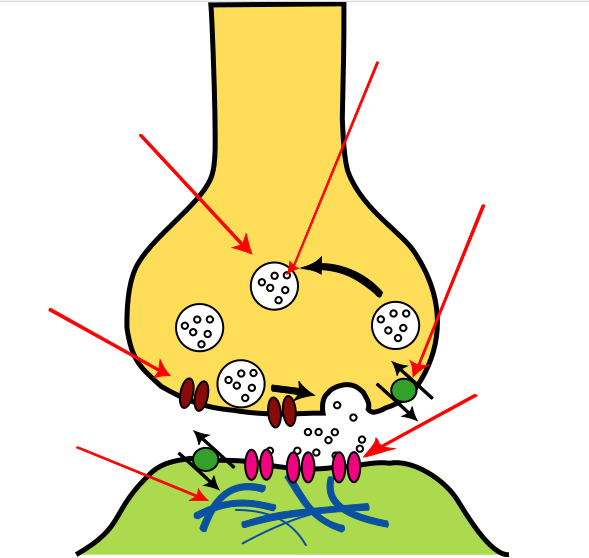
\includegraphics[width = 10cm]{neuroinf_synapse2.png}\\
		& The \textit{synapse} is the cleft between the \textit{presynaptic element} and the \textit{postsynaptic element}.\\
EPSP		& Excitatory postsynaptic potential. Normally, excitatory neurotransmitters open Na$^+$ and K$^+$ channels. Therefore, the conductances for these ions raise, resulting in higher currents, resulting in a change in voltage.\\
IPSP		& Inhibitory postsynaptic potential. Normally, inhibitory neurotransmitters open K$^+$ and Cl$^-$ channels. Therefore, the conductances for these ions raise, resulting in higher currents, resulting in a change in voltage.\\
\textbf{Signal transmission}\\
- At presynaptic element	& \begin{itemize}
                        	  	\item After an \textbf{action potential}, the membrane at the axon terminal is depolarized for a short moment.
					\item Due to the depolarization, voltage-gated \textbf{Ca$^{2+}$-channels} open and Ca$^{2+}$ flows into the presynaptic element.
					\item The increased Ca$^{2+}$ concentration triggers the \textbf{emission of neurotransmitters} into the synaptic cleft.
                        	  \end{itemize}\\
- At postsynaptic element	& \begin{itemize}
                         	  	\item At the postsynaptic element, there are \textbf{ligand-gated ion channels} facing the synapse. The neurotransmitters can ``open'' specific ion channels.
					\item Depending on which ion's channel is opened, an \textbf{EPSP} or \textbf{IPSP} establishes. Mostly, EPSP leads to an increase in membrane voltage, while IPSP mostly lead to a decrease in membrane voltage of the postsynaptic element. Theoretically, EPSP could decrease the membrane voltage, since the channels are opened for both directions
					\item The neurotransmitters are finally removed by enzymes and the membrane voltage levels out again.
                         	  \end{itemize}\\
Electric circuit for synapse	& 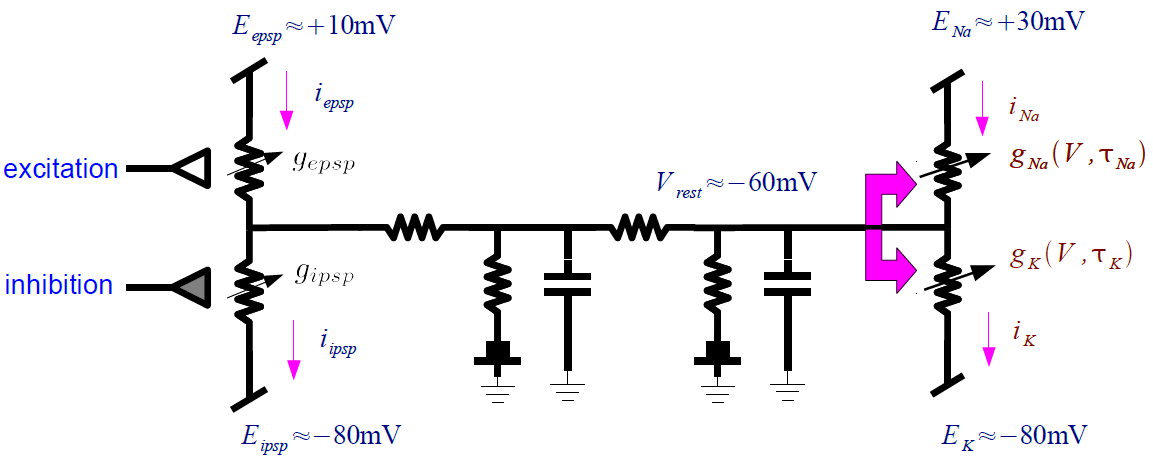
\includegraphics[width = 15cm]{neuroinf_synapse.png}\\
		& The left part is the presynaptic element, the right part is the postsynaptic element. The part in between is in reality repeated many times and represents the leakage.\\
Presynaptic batteries	& $E_{EPSP}$ and $E_{IPSP}$ symbolize the voltages induced by the opening of the ligand-gated ion channels. Therefore, $g_{EPSP}$ and $g_{IPSP}$ depend on ligands (neurotransmitters) and not on voltages. In addition, they are not capable of initiating feedback loops.\\
Postsynaptic batteries	& The already well-known $E_{Na}$ and $E_K$ represent the membrane voltage inside the postsynaptic cell (if their ligand-gated ion channels are closed).\\
Agonist			& An agonist ``enables'' a receptor (of an excitatory or inhibitory ion channel).\\
Antagonist		& An antagonist ``blocks'' a receptor (of an excitatory or inhibitory ion channel).\\
Important neurotransmitter	& \begin{tabular}[t]{ll}
				    Excitatory			& Inhibitory\\\hline
				    Glutamate (always)		& GABA (always except for embryos)\\
				    AMPA (only at specific receptors)\\
				    NMDA (only at specific receptors)\\
				  \end{tabular}\\
\end{longtable}

\section{Lecture 6, Synaptic plasticity and learning}
\begin{longtable}{p{4cm}p{15cm}}
Plasticity	& In this context, plasticity means the ability of synapses to change their properties, such that the synapse is strengthened or weakened.\\
Example		& \begin{tabular}[t]{l}
       		  	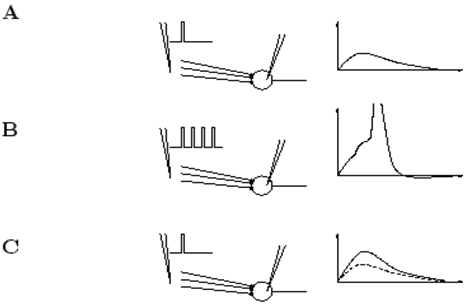
\includegraphics[width=10cm]{neuroinf_plasticity.png}\\
			Left side: Presynaptic spikes. Right side: Postsynaptic potentials\\
			A. Postsynaptic response before modification of synapse
			B. Strong presynaptic stimulation triggers postsynaptic firing
			C. Postsynaptic response after plasticity has occured.
       		  \end{tabular}\\
Hebb's Postulate	& When an axon of cell A is near enough to excite cell B or repeatedly or persistently takes part in firing it, some growth process or metabolic change takes place in one or both cells sucht that A's efficiency, as one of the cells firing B, is increased.\\
Strength of synapse	& The strength of a synapse can be defined by a variety of parameters:\\
			&   \begin{itemize}
			    	\item Neurotransmitter and receptor type (fixed)
				\item Position of synapse
				\item Availability of vesicles
				\item Neuromodulators
				\item Postsynaptic cellular processes
			    \end{itemize}\\
Weight of synapse	& After Hebbian learning, a synpase is strengthened, if presynaptic and postsynaptic cell fire simultaneously. In a neural network, the connection (the synapse) between two artificial neurons has a weight which models the strength of a synapse. For hebbian learning, this weight is defined as $w_{ij} = x_ix_j$ where $x_i, x_j$ are boolean and determine whether or not cell $i$ and $j$ fire for a specific training example.\\
Limitations of Hebbian Learning	& \begin{itemize}
                               	  	\item Only potentiation modeled (no depression)
					\item $\Rightarrow$ Leads to instability (positive feedback loops)
					\item Only variables locally available at the synapse are taken into account
                               	  \end{itemize}\\
Pavlovian Conditioning	& Pavlovian conditioning can be explained by Hebb's postulate: A dog smells food and accumulates saliva, i.e. neuron ``smelling food'' and neuron ``salivation'' are active. By adding a bell to the food, also neuron ``hearing a bell'' is activated. Since neuron ``salivation'' is still active, its synapse with the bell-neuron is strengthened, so that the dog still accumulates saliva, even if the food is taken away.\\
NMDA-Receptor		& \begin{itemize}
				\item Ligand-gated and voltage-gated. The NMDAR is initially blocked by Mg$^{2+}$ ions. It can be unblocked if the postsynaptic membrane is depolarized (by backpropagation, see STDP).
				\item If the channel is unblocked (i.e. on pre- and postsynaptic cell firing simultaneously), Ca$^{2+}$ can flow into the postsynaptic cell.
				\item The presynaptic cell emits Glutamate (agonist) and other Neurotransmitter (coagonists, e.g. glycine) that activate the NMDA channel.
				\item 10x more permeable to Ca$^{2+}$ compared to Na$+$ or K$^+$
				\item Strong / Weak NMDA receptor activation $\Rightarrow$ potentiation / depression of synapse
            		  \end{itemize}\\
AMPA receptor		& \begin{itemize}
				\item Most common receptor in the nervous system.
            		  	\item Unlike the NMDA receptor, the AMPA receptor is not initially blocked.
				\item Unlike NMDAR, AMPAR doesn't allow Ca$^{2+}$ influx.
				\item If the presynaptic cell fires, Glutamate activates the AMPA receptor and Na$^+$ flows into the postsynaptic cell, causing a potential difference which can help to remove the Mg$^{2+}$. But in general, this help alone can't remove the Mg$^{2+}$
				\item Given a Ca$^{2+}$ flux, more AMPA Receptors are built into the synapse, therefore strengthening the connection due to the above mentioned helper role of AMPA receptors.
            		  \end{itemize}\\
Short-term plasticity	& The strengthening or weakening of a synapse lasts for some short time (milliseconds to few minutes) only.\\
LTP			& Long Term Potentiation: A synapse is strengthened in a long time range. Experimentally, the presynaptic cell is made firing with a high frequency (called tetanus). It is then observed, that the EPSP's amplitude is very high for a long time.\\
LTD			& Long Term Depression: A synapse efficiency is weakened in a long time range\\
STDP			& Spike Time Dependent Potentiation: Whether the synapse is strengthened or weakened, is dependent on the time when a spike of the pre- or postsynaptic cell occurs ($Potentiation(t_{pre} - t_{post})$). Example: If the presynaptic cell fires a bit earlier thant the postsynaptic cell, the synapse is strengthened, otherwise weakened. For Hebb's rule, the potentiation is maximal, if $t_{pre} - t_{post} = 0$. STDP adds a temporal factor (or a direction of information) to Hebbian learning: The synapse is strengthened, if the input neuron spikes a little earlier than the output neuron.\\
			& 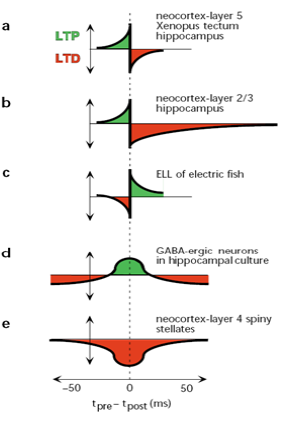
\includegraphics[width = 8cm]{neuroinf_stdp.png}\\
Dopamine		& Dopamine is a drug, which can raise the time range for LTP. Consequently, it is able to change prevent LTD and instead trigger LTP.\\
Factors that influence plasticity	& \begin{itemize}
                                 	  	\item Different plasticity in different brain areas
						\item Diversity in neurons and synapses
						\item Presynaptic spike frequency, postsynaptic membrane voltage, position of dendrites...
						\item Influence of neuromodulators, calcium, drugs, ...
						\item Short-term vs. Long-term effects
                                 	  \end{itemize}

\end{longtable}
\section{Lecture 7, McCulloch Pitts Neuron and Perceptron Learning Algorithm}
\subsection{McCulloch-Pitts Neuron}
\begin{tabular}{p{4cm}p{15cm}}
 States of a neuron	& Only two states: Active (1) or inactive (0)\\
 Electric symbol	& 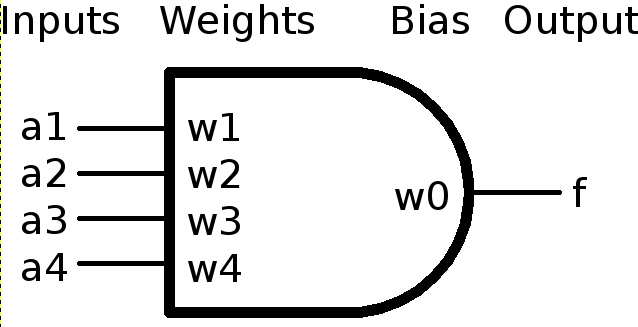
\includegraphics[width = 10cm]{neuroinf_mccullochpitts.png}\\
			& \begin{tabular}[t]{llp{10cm}}
			  Inputs	& bool*		& Input vector represents dendrites. If a presynaptic cell activates a dendrite, the respective vector element is 1.\\
			  Weights	& float*	& Represents efficiency of a synapse. $w < 0$ represents inhibitory signals, $w > 0$ represents excitatory signals.\\
			  Bias		& float		& \\
			  Output	& bool		& $f = \left( \sum_i a_i w_i + w_0 \geq 0 \right)$. The sum represents the soma, which integrates all potentials from the dendrites. $f$ represents whether the neuron spikes or not.
			  \end{tabular}\\
 Examples		& \begin{tabular}[t]{lll}
			    $w = \{1,1\}$	& $-2 < w_o < -1$	& AND-Gate\\
			    $w = \{1,1\}$	& $-1 < w_o \leq -1$	& OR-Gate\\
			    $w = \{-1\}$	& $w = 0$		& NOT-Gate
			  \end{tabular}\\
XOR-Problem		& The XOR-Gate can't be modeled by a single McCulloch Pitts Neuron.\\
Proof			& \begin{tabular}[t]{p{15cm}}
			    Let $(a_1,a_2)$ be the input vector, $(w_1,w_2)$ the corresponding weight vector, $w_0$ the bias and $f$ the output boolean.\\
			    The equation modeling the MCP-Neuron is then $a_1w_1 + a_2w_2 + w_O \geq 0 = f$\\
			    The truth table for the XOR-Gate reads as follows\\
			    \begin{tabular}{|cc|c|}
			    \toprule
			    $a_1$	& $a_2$	& $f$\\\midrule
			    0		& 0	& 0\\
			    1		& 0	& 1\\
			    0		& 1	& 1\\
			    1		& 1	& 0\\\bottomrule
			    \end{tabular}\\
			    The following system of inequalities arises from that truth table\\
			    \begin{tabular}{ccccccc}
			            &   &       &   & $w_0$ & $<$    & 0\\    
			            &   & $w_2$ & + & $w_0$ & $\geq$ & 0\\    
			      $w_1$ &   &       & + & $w_0$ & $\geq$ & 0\\    
			      $w_1$ & + & $w_2$ & + & $w_0$ & $<$    & 0\\
			     \end{tabular}\\
			     By linear combination, one finds that $w_1 + w_2 + 2w_0 \geq 0$ AND $w_1 + w_2 + 2w_0 < 0$ must hold, which is a contradiction.
			   \end{tabular}
\end{tabular}
\subsection{Perceptron learning algorithm}
Folgende �berlegungen liegen der Lernregel des Perzeptrons zu Grunde:
\begin{enumerate}
 \item Wenn die Ausgabe eines Neurons 1 (bzw. 0) ist und den Wert 1 (bzw. 0) annehmen soll, dann werden die Gewichtungen nicht ge�ndert.
 \item Ist die Ausgabe 0, soll aber den Wert 1 annehmen, dann werden die Gewichte inkrementiert.
 \item Ist die Ausgabe 1, soll aber den Wert 0 annehmen, dann werden die Gewichte dekrementiert.
\end{enumerate}
Mathematisch wird der Sachverhalt folgendermassen ausgedr�ckt:\\
Sei $\vec{x}$ der Eingabevektor, $\vec{w}$ der Gewichtsvektor und $0 < \alpha < 1$ der Lerngeschwindigkeits-Koeffizient\\
Eine Gewichtsaktualisierung im Schritt $k$ verl�uft wie folgt:
\begin{enumerate}
 \item $w(k+1) = w(k)$ bei korrekter Ausgabe,
 \item $w_j(k+1) = w_j(k) + \alpha x_{j}$ bei Ausgabe 0 und gew�nschter Ausgabe 1 und
 \item $w_j(k+1) = w_j(k) - \alpha x_{j}$ bei Ausgabe 1 und gew�nschter Ausgabe 0.
\end{enumerate}

\section{Lecture 8, Stretch Reflex}
\subsection{Alpha motor neuron}
\begin{tabular}{p{4cm}p{15cm}}
Function	& $\alpha$-MN innervate skeletal muscle fibers and are directly responsible for their contraction.\\
Location	& They are mainly located in the spinal cord, except for $\alpha$-MN which control head and neck. In the spinal cord, $\alpha$-MNs are located in its gray matter.\\
Fine motor control	& The number of $\alpha$-MNs is directly proportional to the amount of fine control in a muscle.\\
Signaling	& The axons of $\alpha$-MNs are heavily myelinated and are large in diameter to ensure a high speed of the action potential propagation. Unlike most other neurons, $\alpha$-MNs use only acetylcholine as neurotransmitters.
\end{tabular}
\subsection{Stretch Reflex}
\begin{longtable}{p{4cm}p{15cm}}
		& 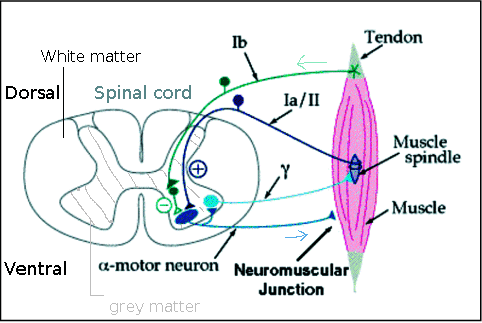
\includegraphics[width=12cm]{neuroinf_stretchreflex.png}\\
		& The stretch reflex is a monosynaptic process, since only a sensory neuron and a motor neuron are involved. There are about 620 muscles in a human body, and about 200 bones. Most of them are in our hands and feet.\\
Process		& \begin{enumerate}
		  	\item Muscle is stretched
			\item Muscle spindle is stretched and its nerve activity increases.
			\item $\alpha$ MN is activated, which causes the spindle to contract. Therefore, the length of the muscle fiber remains constant.
		  \end{enumerate}\\
Examples	& \begin{enumerate}
        	  	\item Leaning on a side
			\item Biceps reflex
			\item Knee-jerk reflex
        	  \end{enumerate}\\
Axon lengths	& \begin{tabular}[t]{ll}
		    White matter	& Grey matter\\\hline
		    4km / mm$^3$	& 9m / mm$^3$\\
		    Not myelinated	& Myelinated\\
		    Long distance, low bandwidth
		  \end{tabular}
\end{longtable}


\section{Lecture 9, Synaptic activation}
\subsection{Dispute over transmission type}
\begin{tabular}{p{4cm}p{15cm}}
Chemical transmission	& Otto Loewi 1921: Experiment on vagus nerve / frog heart proves that a chemical substance is responsible for transmission of nerve impulse. Henry Dale later identified this substance as Acetylcholine. The neurotransmitter acted inhibitory, i.e. the heart rate slowed down if the impulse was transmitted.\\
Electrical transmission	& J. Eccles argues the transmission must be of electrical nature, because the chemical transmission (diffusion) would take too long. He later falsified his own theory\\
\end{tabular}\\
\begin{tabular}{p{4cm}p{15cm}}
Neurotransmission	& \begin{enumerate}
                 	  	\item Action potential is triggered and comes down the axon (presynaptic cell)
				\item Vesicles which are already docked at the synapse might release its neurotransmitters into the synapse.\newline
				      The number of neurotransmitters per vesicle is roughly about 1000
                 	  \end{enumerate}\\
Depolarization potential	& 0.1 - 0.3 mV per synapse $\Rightarrow$ If (Action potential threshold) - (Resting potential) = 40mV, then about 133 - 400 synapses need to fire\\
\end{tabular}\\
\subsection{Activation of muscular cells}
\begin{tabular}{p{4cm}p{15cm}}
Activation	& Recall: A \textbf{single} synapse activates the action potential of a muscle, unlike central synapses, where only many synapses together can trigger an action potential.\\
Reasons		& \begin{itemize}
       		  	\item Giant synapse with many vesicle releasers and receptors. 
			\item In a neuromuscular synapse, many vesicles can be released simultaneously (Central synapses often release only one vesicle). A vesicle has a specific number of neurotransmitters which it releases.
       		  \end{itemize}\\
Muscle control	& \begin{itemize}
			\item Finesse of muscular control depends on number of motor neurons.
			\item The more motor neurons, the more muscle fibers there are.
              	  \end{itemize}\\
\end{tabular}\\
\begin{tabular}{p{4cm}p{15cm}}
Influencing plasticity	& \begin{itemize}
          	  	\item Probability of firing (has to do with Ca$^{2+}$ concentrations), presynaptic
			\item Number of synapses, presynaptic
			\item Number of receptors, postsynaptic
          	  \end{itemize}
\end{tabular}
\section{Lecture 10, Neural Coding}
Problem of neural coding: A single neuron spikes in a probabilistic way. Neglecting the duration of an action potential (~1ms) and differences in maximal amplitude and shape, action potentials can be stereotyped and therefore be thought of as a random variable. Therefore, statistical methods are needed to get meaningful statements. In the following, a ``run'' refers to a random experiment, in which a neuron can respond (several times) to a stimulus.
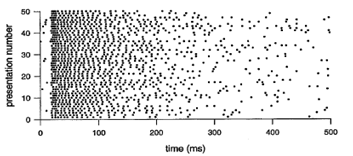
\includegraphics[width=10cm]{neuroinf_spikeruns.png}\\
Abbreviation: (S$|$M)N(S$|$M)R = (Single$|$Multiple) Neuron, (Single$|$Multiple) Run\\
\subsection{Neuronal Rate Codes}
Neuronal rate codes rely on the spike rate as information carrier. The different methods show how such a rate can be computed.\\
\begin{longtable}{p{4cm}p{15cm}}
Neuronal gain function (SNSR)	& Output spike rate = f(input current). The mean spike rate is determined by a temporal average over the spikes of a neuron in a run.\\
Peri-Stimulus Time Histogram (SNMR)	& Average over several runs. No temporal average is taken. The probability of a spike ($\Leftrightarrow$ firing rate) depends on the time.\\
Rate as a function of stimulus	& 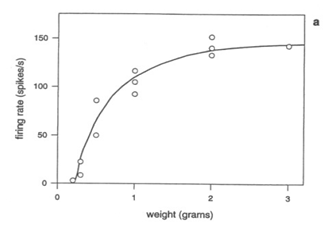
\includegraphics[width=10cm]{neuroinf_ratestimulus1.png}\\
Adaption to stimulus		& 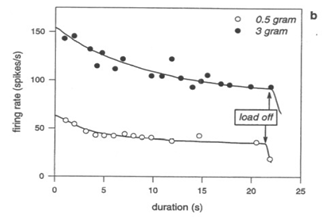
\includegraphics[width=10cm]{neuroinf_ratestimulus2.png}\\
\textbf{Tuning curves}		& Neurons of any kind often have a preferred stimulus, i.e. the spike rate is extraordinarily high for a certain stimulus. E.g. the peak firing rate of the ``blue'' photoreceptor in the retina is for wavelengths around 450 nm (blue color) or head direction cells in rats or ``Jennifer Aniston cells'' That means, a neuron can encode a certain (very exact) information.\\
What can a single neuron encode (examples)	& \begin{itemize}
                               	  	\item Placement (Rat hippocampus): Fires whenever rat enters a particular region in its environment
					\item Head-direction: Fires whenever rat's head points to a specific direction (compass)
					\item Anything about Jennifer Aniston
                               	  \end{itemize}\\
Topographic maps		& In the CNS, many neurons which have similar preferred stimuli, are grouped together, i.e. the distances between them are small. For example, there are topographic maps for the visual system, the auditotory system and so on. It makes sense that the neurons build clusters between neurons which will be highly interconnected.\\
Pros and Cons			& \begin{tabular}[t]{p{7cm}p{7cm}}
				    +: Easy to understand and measure	& -: No timing effects\\
									& -: The behavioural response time is shorter than the integration time\\
									& -: Tuning curves might be misleading, because more than one stimulus could be encoded.
				  \end{tabular}\\
\end{longtable}
\subsection{Population Rates (MNSR)}
\begin{tabular}{p{4cm}p{15cm}}
Population	& A population is a family of neurons which react to the same type of stimulus but have different peak reactions. (e.g. Photoreceptor cells) As an individual neuron is too noisy and therefore unreliable, a population of neurons levels out these noises statistically.\\
Rate		& The rate is determined by an average over equivalent neurons in a single run.\\
Statistics	& For the photoreceptor cells for example, it makes no sense to average over the firing rates. Rather an average over the encoded information (the color wavelength), weighted with the photoreceptor's spike rate is meaningful. (E.g. Activation of S and L photoreceptor results in a color somewhere on the purple line)\\
Examples	& Neuron for sensing movement directions, neuron for sensing wind directions
\end{tabular}
\subsection{Neuronal Event Codes}
Sometimes, the precise timing of a spike encodes information (for example spike-time-dependent plasticity). Then, coding relying solely on firing rates is insufficient. Therefore, neuronal event codes depend on the timing of spikes.\\
\begin{tabular}{p{4cm}p{15cm}}
Time-to-first-spike codes	& Instead of a firing rate, the time to the first spike is the information carrier. Relationship to rate codes: High rate implies fast firing\\
Pros and Cons			& \begin{tabular}[t]{p{7cm}p{7cm}}
				    +: Very fast and efficiently measured	& -: Requires reference signal\\
										& -: Susceptible to noise\\
				  \end{tabular}\\
Local field potential		& Dominated by dendritic synaptic activity, reflects the integration of membrane currents in a local region. Interesting if LFP high, but no firing takes place.\\
\end{tabular}
\subsection{Stimulus reconstruction}
\begin{itemize}
	\item Whole stimulus reconstruction may not be relevant.
	\item Particular features may be encoded better (more precisely by a neuron, e.g. ``Jennifer Aniston Neuron'') than others.
	\item Cells may respond to only particular aspects of stimulus.
	\item Or respond to multiple aspects of stimulus.
	\item Artificial stimuli used for studies may be predictable.
\end{itemize}
\section{Lecture 11: Hopfield Networks}
\begin{longtable}{p{4cm}p{15cm}}
Hopfield Network	& 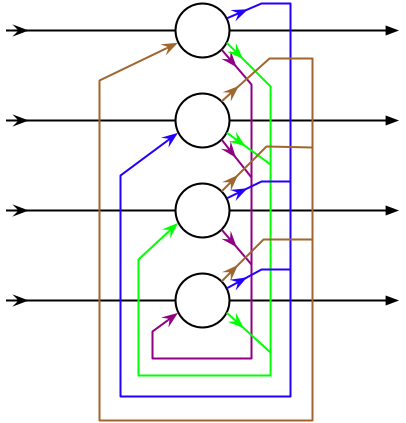
\includegraphics[width=10cm]{neuroinf_hopfieldnet.png}\\
Usage of Hopfield Network	& The Hopfield Network models \textbf{associative memory}. Given a initial state, the Hopfield Network converges to some stable state, which is similar to the initial state, whatever similar means. Memory by association (i.e. similarity) is a fundamentally different concept than memory by list lookup as it is done in computers.\\
Memory concepts		& \begin{tabular}[t]{lrcl}
			    Human:	& Initial input		& $\xrightarrow[]{Association}$	& Memorized information\\
			    Computer:	& Input index		& $\xrightarrow[]{List lookup}$	& Memorized information	
			  \end{tabular}\\
Nodes			& The nodes represent neurons, which can be modelled by McCulloch-Pitts Neurons, as an example. A neuron can either be active (1) or inactive (0, sometimes -1)\\
			& Let the activation state be denoted by $a_i$.\\
Edges			& An edge represent a connection between two neurons. The strength of an edge is modeled by its weight.\\
			& Let the weight of an edge be denoted by $w_{ij}$\\
Pattern			& The set of each node's state is called a pattern (i.e. 0000111110100).\\
Assumptions		& \begin{itemize}
           		  	\item No autoconnections.
				\item Weights between two neurons are the same (symmetric weights)
           		  \end{itemize}\\
Bias			& The bias is neglected. For computations, a extra neuron can be imposed which has a weight equal to the bias and which is always active.\\
Theorem			& A Hopfield network always converges to a stable configuration.\\
Energy			& $-\frac{1}{2} \sum_{i,j} w_{i,j} a_i a_j$ (if $a_i \in \{0,1\}$)\\
``Proof''		& We can define an algorithm according to which the energy must be minimized. That is, starting from an arbitrary initial condition, a neuron will be activated, if its weights contribute nonnegatively to the energy. This asynchronous update converges.\\
Update rule		& If the sum of all edges from activated nodes to the node to be updated is nonnegative, this node will be activated (value 1 is assigned). Otherwise it will be inactivated (valu 0 or -1). This update rule is applied to all nodes asynchronously (overall state can change from node to node) or synchronously (equal state for all nodes). For asynchronous updates, the update order influences the result.\\
Relation to Max-Flow-Min-Cut	& To minimize the energy, we want to ``remove'' edges with a very low (or even negative) weight. This can be done by finding the minimal cut of the Hopfield network and then inactivate all nodes on one side of the cut. The side with less nodes should be chosen.\\
Learning rules		& Learning a pattern means lowering its energy. In fact, a pattern to be remembered must be a local minimum. This can be achieved by adjusting the weights in such a way that the desired pattern has a minimal energy. One possible learning rule is Hebbian learning.\\
Hebbian learning	& \begin{tabular}[t]{l}
			    $w_{ij} = \frac{1}{N} \sum_{\mu=1}^p \epsilon_i^{\mu} \epsilon_j^{\mu}$
			    $N$: Number of neurons\\
			    $p$: Number of patterns to learn\\
			    $\epsilon_i^{\mu}$: State of bit $i$ of pattern $\mu$
			  \end{tabular}\\
Role of assumptions	& If the assumptions are broken, there are easy cases which lead to infinite cycling.\\
\end{longtable}
\section{Lecture 12: Feed-forward neural networks and Back-propagation}
\begin{tabular}{p{4cm}p{15cm}}
				& 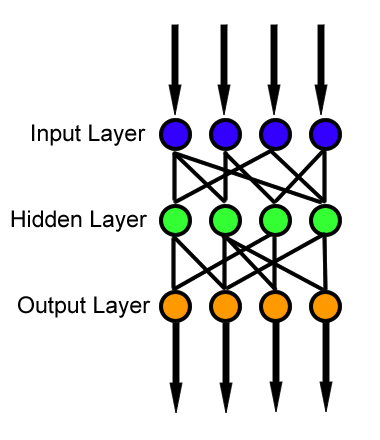
\includegraphics[width=10cm]{neuroinf_feedforward.png}\\
Feed-forward neural network	& In contrast to a recurrent neural network such as a Hopfield network, a FFNN, the connections between the neurons do not form a cycle. In a FFNN, information has only one direction: forward\\
Definitions		& \begin{tabular}[t]{l}
			    Let $N$ be the number of input signals\\
			    Let $D$ be the number of different input signals\\
			    Let $\vec{x}$ be the set of input signals (length $N$)\\
			    Let $\vec{f}$ be the set of network outputs (length $D$)\\
			    Let $\vec{g}$ be the set of desired network outputs (length $D$)
			  \end{tabular}\\
Error			& $E = \sum_i(f_i-g_i)^2$\\
Sigmoid function	& The output $f$ of an artificial neuron is given by $f = \mathrm{sgn} ( \mathbf{w^T x} + b)$, where $\mathbf{x}:$ inputs, $\mathbf{w}:$ weights, $b$: bias and assuming the boolean output is set as $f = \{-1,1\}$. Since the signum function is not continuous and not differentiable (?), we replace the signum function by the sigmoid function $f(y) = \frac{1}{1 + e^{-y}}$. The derivative of the sigmoid function is $\frac{df}{dy} = \frac{e^{-y}}{(1+e^{-y})^2} = y(1-y)$\\
Algorithm		& \begin{algorithmic}
			    \For {i = 0; i $<$ D; i++}
				\State Feed input $(\vec{x})_i$ to network. Compute $f_i - g_i$
				\For{each weight $w_k$}
				  \State Compute sensitivity of output: $\frac{df_i}{dw_k}$
				  \State $w_k = w_k-\epsilon (f_i-g_i) \frac{df_i}{dw_k}$ ($\epsilon$ is the learning rate)
				\EndFor
			    \EndFor
			  \end{algorithmic}\\
\end{tabular}

\subsection{Einheiten und Zeichen}
\begin{tabular}{p{8cm} p{2cm} p{4cm} p{4cm}}
Gr�sse			& Symbol	& Bezeichnung der Einheit	& SI-Gr�sse\\\midrule
L�nge			& $l$		& Meter				& m\\
Masse			& $m$		& Kilogramm			& kg\\
Zeit			& $t$		& Sekunde			& s\\
Geschwindigkeit		& $v$		&				& ms$^{-1}$\\
Beschleunigung		& $a$		&				& ms$^{-2}$\\
Frequenz		& $\nu$		& Hertz (Hz)			& s$^{-1}$\\
Arbeit			& $W$		& Joule (J)			& m$^2$ kg s$^{-2}$\\
Leistung		& $P$		& Watt (W)			& m$^2$ kg s$^{-3}$\\
Energie			& $U,E$		& Joule (J)			& m$^2$ kg s$^{-2}$\\
Temperatur		& $T$		& Kelvin (K)			& m$^2$ kg s$^{-2}$ / Teilchen\\
Elektrischer Strom	& $I$		& Amp�re (A)			& A\\
Ladung			& $q,Q$		&				& C = A s\\
Elektrische Spannung	& $V$		& Volt (V)			& m$^2$ kg s$^{-3}$ A$^{-1}$\\
Elektrische Kapazit�t	& $F$		& Farad (F)			& C V$^{-1}$\\
Elektrischer Widerstand	& $\Omega$	& Ohm ($\Omega$)		& V A$^{-1}$\\
Elektrische Leitf�higkeit	& $g,S$	& Siemens (S)			& V$^{-1}$ A\\
Elektrisches Feld	& $\epsilon$	& 				& m kg s$^{-3}$ A$^{-1}$\\
Stromdichte		& $j$		&				& m$^{-2}$ A\\
Magnetfeld		& $B$		& Tesla (T)			& kg s$^{-2}$ A$^{-2}$\\
\end{tabular}

\end{document}